\documentclass[aspectratio=169]{beamer}

% because we need to claim weird things
\newtheorem{claim}{Claim}
\newtheorem{defn}{Definition}
%\newtheorem{lemma}{Lemma}
\newtheorem{thm}{Theorem}
\newtheorem{vita}{Vit\ae}
\newtheorem{qotd}{Quote of the Day}

\usepackage{algorithm}
\usepackage{algpseudocode}
\usepackage{listings}
\usepackage{color}
\usepackage{graphics}
\usepackage{ulem}
\bibliographystyle{unsrt}

% background image
\usebackgroundtemplate%
{%
    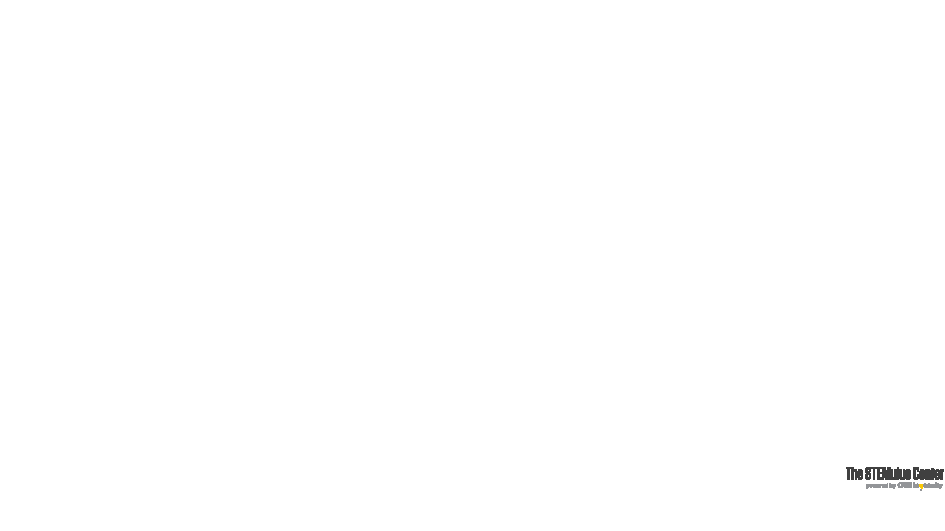
\includegraphics[width=\paperwidth,height=\paperheight]{../artifacts/stemulus.pdf}%
}
\setbeamertemplate{caption}[numbered]
\lstset{%
	breaklines=true,
	captionpos=b,
	frame=single,
	keepspaces=true,
	showstringspaces=false
}

% page numbers
\addtobeamertemplate{navigation symbols}{}{%
    \usebeamerfont{footline}%
    \usebeamercolor[fg]{footline}%
    \hspace{1em}%
    \insertframenumber/\inserttotalframenumber
}

% presentation header
\usetheme{Warsaw}
\title{Introduction to mySQL}
\author{Dylan Lane McDonald}
\institute{CNM STEMulus Center\\Web Development with PHP}
\date{\today}

\begin{document}
\lstset{language=Java}
\begin{frame}
\titlepage
\end{frame}

\begin{frame}
\frametitle{Outline}
\tableofcontents
\end{frame}

\section{Set Theory}
\begin{frame}
\frametitle{Set Theory}
A \textbf{set} is a collection of distinct objects. Sets and their operations serve as a mathematical motivation to how databases store, access, and relate data.
\begin{table}
\begin{tabular}{|l|l|l|}
\hline
\textbf{Operation} & \textbf{Name} & \textbf{Comment}\\
\hline
$A \cap B$ & Intersection & All items in common in $A$ \& $B$\\
\hline
$A \cup B$ & Union & All items in $A$ \& $B$\\
\hline
$A \times B$ & Cartesian Product & All items in $A$ paired with $B$\\
\hline
$A \backslash B$ & Compliment & All items in $A$ not in $B$\\
\hline
$A \subset B$ & Subset & All items in $A$ exist in $B$\\
\hline
$\left| A \right|$ & Cardinality & Number of items in $A$\\
\hline
$x \in A$ & Element Of & $x$ exists in $A$\\
\hline
\end{tabular}
\caption{Set Operations}
\label{tbl:setoperations}
\end{table}
\end{frame}

\begin{frame}
\frametitle{Example Set Operations}
Let $A = \{1, 2, 3\}$ and $B = \{3, 4, 5\}$.
\begin{align*}
A \cap B &= \{3\}\\
A \cup B &= \{1, 2, 3, 4, 5 \}\\
A \times B &= \{(1, 3), (1, 4), (1, 5), (2, 3), (2, 4), (2, 5), (3, 3), (3, 4), (3, 5)\}\\
A \backslash B &= \{1, 2\}\\
A \subset B &= \textnormal{false}\\
\left| A \right| &= 3\\
2 \in A &= \textnormal{true}
\end{align*}
These examples of all the operations in Table \ref{tbl:setoperations} will motivate how to visualize database operations and queries.
\end{frame}

\begin{frame}
\frametitle{Common Sets}
\begin{table}
\begin{tabular}{|l|l|}
\hline
\textbf{Set} & \textbf{Comment}\\
\hline
$\emptyset$ & Empty set $ = \{\}$\\
\hline
$\mathbb{P}$ & Prime numbers $ = \{2, 3, 5, \dots\}$\\
\hline
$\mathbb{N}$ & Natural numbers $ = \{1, 2, 3, \dots \}$\\
\hline
$\mathbb{Z}$ & Integers $ = \{\dots, -2, -1, 0, 1, 2, \dots\}$\\
\hline
$\mathbb{Q}$ & Rational numbers (all numbers $\frac ab$ where $b \ne 0$)\\
\hline
$\mathbb{R}$ & Real numbers (all numbers without a complex part)\\
\hline
$\mathbb{C}$ & Complex numbers (all numbers in the form $a + bi$)\\
\hline
\end{tabular}
\caption{Common Sets}
\label{tbl:commonsets}
\end{table}
Note the row above is a subset of the row below in Table \ref{tbl:commonsets}. i.e.,
\[
\emptyset \subset \mathbb{P} \subset \mathbb{N} \subset \mathbb{Z} \subset \mathbb{Q} \subset \mathbb{R} \subset \mathbb{C}
\]
\end{frame}

\section{Introduction to Relational Database Management Systems}
\subsection{Introduction to Relational Database Management Systems}
\begin{frame}
\frametitle{Introduction to Relational Database Systems}
\begin{defn}
\textbf{Relational Database Management Systems} (RDBMS) are systems that store and relate data using first order predicate logic. RDBMS allow concurrent access to the same data and maintain the integrity and relations of the data they contain.
\end{defn}

\pause
\mbox{}\\
The key to RDBMS's success is the relationships shared among all the entities in the database, making the database flexible and searchable. The relations give multiple deterministic, efficient paths to the data required.
\end{frame}

\begin{frame}
\frametitle{RDBMS Elements}
RDBMS have the following elements:
\begin{enumerate}
	\item \textbf{Database}: In this context, a database is a collection of related entities.
	\item \textbf{Entity}: A particular \emph{model} in a database. This is typically a \emph{class} in an object oriented program. This is a \emph{set} in set theory.
	\item \textbf{Row}: A specific member of an entity. This is an \emph{object} in object oriented programming. This is an \emph{element} in set theory.
	\item \textbf{Attribute}: A specific field of an entity. This is a \emph{state variable} in object oriented programs.
	\item \textbf{Relation}: A relationship two entities have on one or more attributes. This is implemented as a \emph{method} in object oriented programming.
\end{enumerate}
\end{frame}

\subsection{Indexes \& Keys}
\begin{frame}
\frametitle{Indexes \& Keys}
\begin{defn}
An \textbf{index} on an attribute in an entity is a data structure that makes it faster to search through rows using one or more inputs. 
\end{defn}
\begin{defn}
A \textbf{key} an index that uniquely identifies a row in an entity. If the key is the main identifier for the row, it is known as a \textbf{primary key}.
\end{defn}
\mbox{}\\
Every entity should have a primary key defined. The primary key is critical in disambiguating among the other rows as well as serving as the typical identifier for relations.
\end{frame}

\subsection{Relations}
\begin{frame}
\frametitle{Relations}
\begin{defn}
A \textbf{relation} is a semantically defined link between two entities. The relation will occur on one or more attributes.
\end{defn}
\mbox{}\\
The three types of relations are:
\begin{enumerate}
	\item 1-to-1: where one row in an entity refers to another entity and gets 0 or 1 results.
	\item 1-to-$n$: where one row in an entity refers to another entity and gets 0 or more results.
	\item $m$-to-$n$: where \emph{multiple rows} can refer to another entity and get 0 or more results.
\end{enumerate}
\end{frame}

\begin{frame}
\frametitle{Facebook Relations}
Consider a small cross-section of Facebook as an example database. Suppose we have the following entities:
\begin{itemize}
	\item \textbf{User}: A user's username \& password.
	\item \textbf{Timeline}: A user's posts, photos, etc.
	\item \textbf{Groups}: A group of users with common interests.
\end{itemize}
\mbox{}\\
The relations in our small Facebook database would be:
\begin{itemize}
	\item 1-to-1: One user can have only one timeline.
	\item 1-to-$n$: One user can post $n$ items to her/his timeline.
	\item $m$-to-$n$: Many users can belong to multiple groups.
\end{itemize}
\end{frame}

\section{SQL}
\subsection{Core Operations}
\begin{frame}
\frametitle{Core SQL Operations}
The core SQL operations are:
\begin{itemize}
	\item \textbf{Select}: Extract row(s) from an entity based on search criteria.
	\item \textbf{Update}: Update row(s) in an entity based on search criteria.
	\item \textbf{Delete}: Delete row(s) from an entity based on search criteria.
	\item \textbf{Insert}: Insert a new row into an entity.
\end{itemize}

\mbox{}\\
These four operations are at the core of any SQL-aware application. In the Model-View-Controller design pattern, these four operations are the ones that are repeated continuously. In fact, in accordance of the \href{https://www.owasp.org/index.php/Least_privilege}{Principle of Least Privilege}, most database users are limited to these four operations.
\end{frame}

\subsection{Joins}
\begin{frame}
\frametitle{Joins}
\begin{defn}
A \textbf{join} is the process of gathering data from two entities. A join is executed on a field that is common to both entities.
\end{defn}
\mbox{}\\
The major types of joins are:
\begin{itemize}
	\item \textbf{Inner Join}: All rows where field $x$ is common to $A$ and $B$ - $A \cap B$
	\item \textbf{Left Outer Join}: All rows where field $x$ is in $A$ and not in $B$ - $A \backslash B$
	\item \textbf{Right Outer Join}: All rows where field $x$ is in $B$ and not in $B$ - $B \backslash A$ 
\end{itemize}
\end{frame}
\end{document}
